\chapter{Vorlesung}
\section*{Universelles Hashing (Fortsetzung)}
Könnte ein boshafter Mitspieler n Schlüssel bei gegebener fester Hashfunktion wählen, so würde er solche wählen, die auf den gleichen Slot unter gegebener Hashfunktion abgebildet werden. $\rightsquigarrow$ Durchschnittliche Ablaufzeit von $O(n)$
\paragraph{Idee} zufällige Wahl der Hashfunktion aus einer Familie von Funktionen derart, dass die Wahl unabhängig von den zu speichernden Schlüssel ist (universelles Hashing).
\subsection{Definition}
Sei $\mathcal{H}$ eine endliche Menge von Hashfunktionen, welche ein gegebenes Universum $U$ von Schlüsseln auf $\{ 0,\ldots,m-1 \}$ abbildet. Sie heißt universell, wenn für jedes Paar von Schlüsseln $k,l\in U~~l\neq k$ die Anzahl der Hashfunktionen $h\in \mathcal{H}$ mit $h(l)=h(k)$ höchstens $\frac{|\mathcal{H}|}{m}$. Anders: Für ein zufälliges $h\in\mathcal{H}$ beträgt die Wahrscheinlichkeit, dass zwei unterschiedliche Schlüssel $k,l$ kollidieren, nicht mehr als $\frac{1}{m}$.
\subsection{Beispiel}
$p$ Primzahl, so groß, dass alle möglichen Schlüssel $k\in U$ im $0,\ldots,p-1$ liegen. $\mathbb{Z}/p\mathbb{Z}$ bezeichnet den Restklassenring $\mod{p}$ (weil $p$ prim, ist $\mathbb{Z}/p\mathbb{Z}$ ein Körper).
$\mathbb{Z}/p\mathbb{Z}^*$ ist die Einheitengruppe.
\paragraph{Annahme:} Die Menge der Schlüssel im Universum $U$ ist größer als die Anzahl der Slots in der Hashtabelle. Für $a\in \mathbb{Z}/p\mathbb{Z}^*$ und $b\in \mathbb{Z}/p\mathbb{Z}$ betrachte:
\[ h_{a,b}(k) := (a\cdot k + b \mod{p})\mod{m} ~~~(*)\]
Damit ergibt sich die Familie
\[ \mathbb{Z}/p\mathbb{Z}^*=\{ 1,\ldots,p-1 \}~~\mathbb{Z}/p\mathbb{Z}=\{ 0,\ldots,p-1 \}~~ \mathcal{H}_{p,m}=\{h_{a,b}|a\in \mathbb{Z}/p\mathbb{Z}^*, b \in\mathbb{Z}/p\mathbb{Z}^{(*)}~~|\mathcal{H}|=p(p-1)  \} \]
\paragraph{Satz}
Die in $(*)$ eingeführte Klasse von Hashfunktionen ist universell.
\paragraph{Beweis}
Seien $k,l$ Schlüssel auf $\mathbb{Z}/p\mathbb{Z}$ mit $k\neq l$\\
Für $h_{a,b}\in \mathcal{H}_{p,m}$ betrachten wir
\[ r=(a\cdot k+b)\mod{p} \]
\[ s=(a\cdot l+b)\mod{p} \]
Es ist $r \neq s$\\
Dazu:
\[ r-s = a\cdot(k-l) \mod{p} ~~~(*2)\]
\paragraph{Angenommen $r-s=0$}
\[ 0=a\cdot(k-l)\mod{p}\text{, aber }a\in\mathbb{Z}/p\mathbb{Z}^* \Rightarrow a\neq 0\text{ und } k\neq l \Rightarrow k-l\neq 0 \]
Da $p$ prim ist $\mathbb{Z}/p\mathbb{Z}$ ein Körper $\Rightarrow$ kein Nullteiler $\Rightarrow a\cdot (k-l)\neq 0\Rightarrow r\neq s$\\
Daher bilden $h_{a,b}\in \mathcal{H}_{p,m}$ unterschiedliche Schlüssel $k,l$ auf unterschiedliche Elemente ab. ("`Auf dem level $\mod{p}$"' gibt es keine Kollisionen).\\
Aus $(*2)$ folgt:
\[ (r-s)(k-l)^{-1} = a\mod{p} \]
\[ r-a\cdot k = b\mod{p} ~~\text{Bijektion zwischen (k,l) und (a,b)}\]
Daher ist die Wahrscheinlichkeit, dass zwei Schlüssel $h\neq l$ kollidieren, gerade die Wahrscheinlichkeit, dass $r\equiv s \mod{m}$, falls $r\neq S$ zufällig gewählt (aus $\mathbb{Z}/p\mathbb{Z}$).\\
Für gegebenes $r$ gibt es unter den übrigen $p-1$ Werten für $s$ höchstens $\lceil \frac{p-1}{m} \rceil \leq \lceil \frac{p}{m} \rceil -1$ Möglichkeiten, sodass $s\neq r\mod{p}$ aber $r=s\mod{m}$
\subsection{Abschätzung nach oben}
\[\lceil \frac{p}{m} \rceil -1  \leq \frac{(p+m-1)}{m}-1 = \frac{p-1}{m} \text{ Kollisionsmöglichkeiten} \]
Die Wahrscheinlichkeit, dass $r$ und $s$ kollidieren $\mod{m}$ Kollisionsmöglichkeiten / Gesamtzahl der Werte
\[ =\frac{p-1}{m}\cdot\frac{1}{p-1}=\frac{1}{m} \]
$\Rightarrow$ Für ein Paar von Schlüsseln $k,l\in \mathbb{Z}/p\mathbb{Z}$ mit $k\neq l$
\[ P[h_{a,b}(k)=h_{a,b}(l)] \leq \frac{1}{m} \Rightarrow \mathcal{H}_{p,m} \text{ universell!} \]
\section{Perfektes Hashing}
\paragraph{Wichtig}
Menge der Schlüssel ist im Vorhinein bekannt und ändert sich nicht mehr.
\paragraph{Beispiele}
reserved words bei Programmiersprachen, Dateinamen auf einer CD
\subsection{Definition}
Eine Hashmethode heißt perfektes Hashing, falls $O(1)$ Speicherzugriffe benötigt werden, um die Suche nach einem Element durchzuführen.
\paragraph{Idee}
Zweistufiges Hashing mit universellen Hashfunktionen.
\begin{enumerate}
	\item Schritt  $n$ Schlüssel, $m$ Slots durch Verwendung der Hashfunktion $h$, welche aus einer Familie universeller Hashfunktionen stammt.
	\item Schritt  Statt einer Linkedlist im Slot anzulegen, benutzen wir eine kleine zweite Hashtabelle $S_j$ mit Hashfunktion $h_j$
\end{enumerate}
\paragraph{Bild} Schlüssel $k=\{ 10, 22, 37, 49, 52, 60, 72, 75 \}$\\
Äußere Hashfunktion $h(k)=((a\cdot b) \mod{p})\mod{m}$
\[ a=3,~~b=42,~~p=101,~~m=9 \]
\[ h(10)= \underset{=72}{ \underbrace{ (3\cdot 10+42\mod101) } }\mod{9}=0 \]
\begin{figure}[h]
\centering
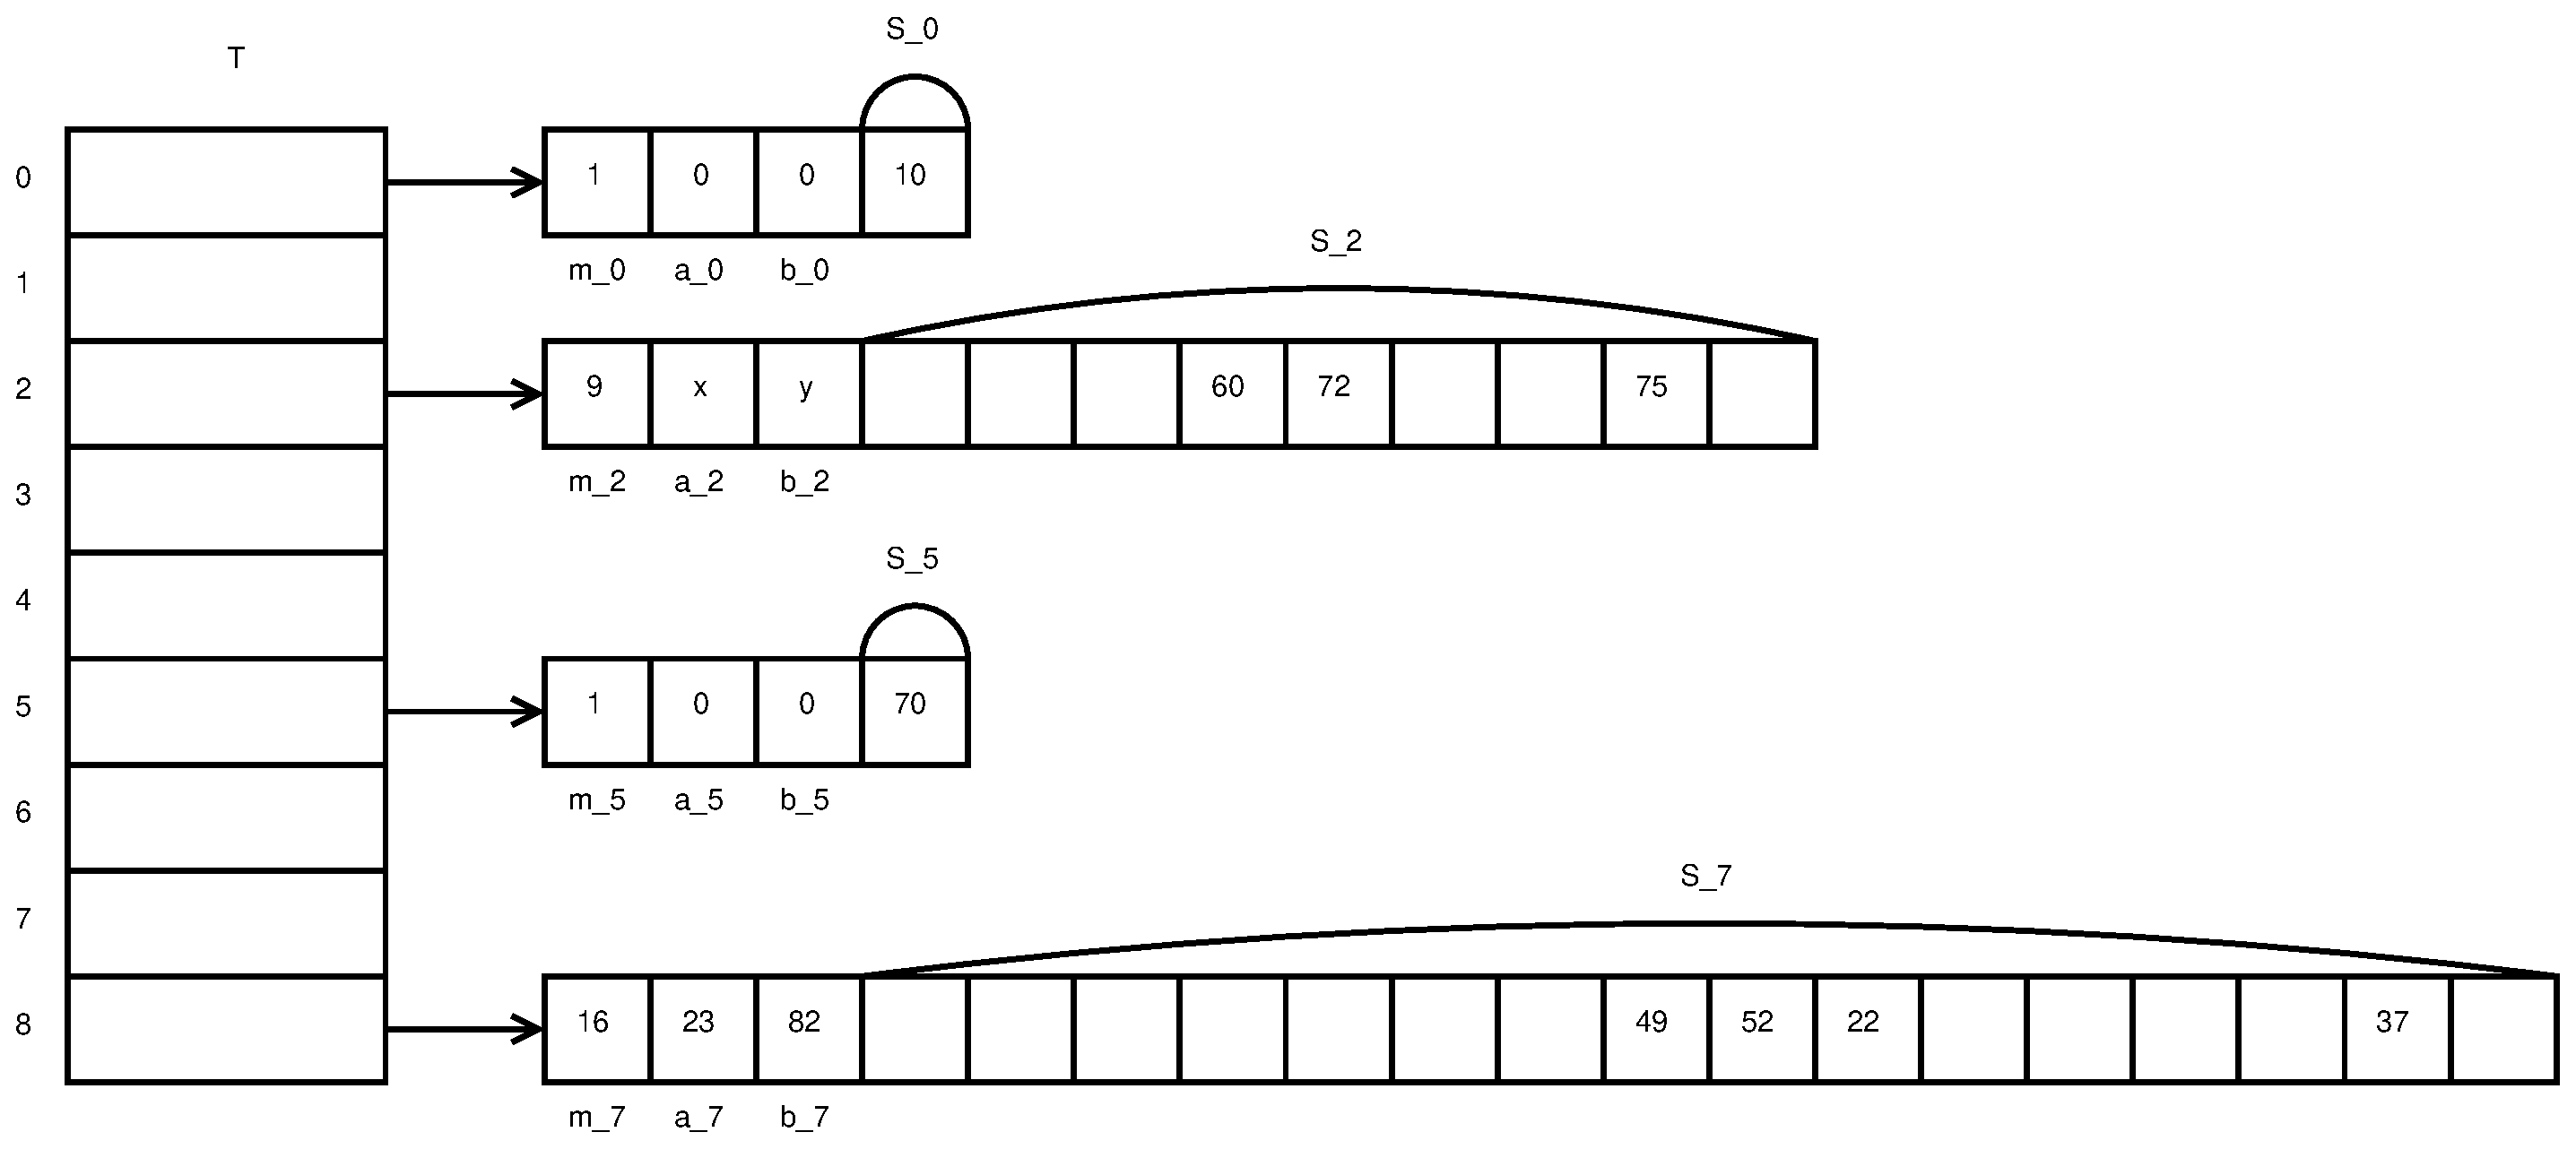
\includegraphics[width=0.7\linewidth]{14/Grafik/Hashing}
\caption{Perfekte Hashtabelle}
\label{fig:Hashing}
\end{figure}
Um zu garantieren, dass keine Kollision auf der zweiten Ebene auftreten, lassen wir die Größe von $S_j$ gerade $n_j^2$ sein ($n_j\neq \#$Schlüssel$\mapsto j$Slot).\\
Wir verwenden für die Hashfunktion der ersten Ebene eine Funktion aus $\mathcal{H}_{p,m}$. Schlüssel die im j-ten Slot werden in der sekundären Hashtabelle $S_j$ der Größe $m_j$ mittels $h_j$ gehasht.  $h_j\in\mathcal{H}_{p,m}$
\paragraph{Wir zeigen:} 2 Dinge:
\begin{enumerate}
	\item Wie versichern wir, dass die zweite Hashfunktion keine Kollision hat.
	\item Der erwartete Speicherbedarf ist $O(n)$
\end{enumerate}
\paragraph{zu 1.}
\subparagraph{Satz}
Beim Speichern von $n$ Schlüsseln in einer Hashtabelle der Größe $m=n^2$ ist die Wahrscheinlichkeit, dass eine Kollision auftritt $<\frac{1}{2}$
\subparagraph{Beweis:}
Es gibt $\binom{n}{2}$ mögliche Paare, die kollidieren können. Jedes kollidiert mit der Wahrscheinlichkeit $\leq \frac{1}{m}$, falls $h\in\mathcal{H}$ zufällig gewählt wurde.\\
Sei $X$ eine zufallsvariable(ZV), $X$ zählt Kollisionen:\\
Für $m=n^2$ ist die erwartete Zahl der Kollisionen:
\[ E[X]=\binom{n}{2}\cdot\frac{1}{m}=\binom{n}{2}\cdot\frac{1}{n^2}=\frac{n!}{2!(n-2)!n^2}=\frac{(n-1)}{2n}\leq\frac{1}{2} \]
Anwenden der Markow-Ungleichung (a=1):
\[ P[X\geq 1]\leq \frac{E[X]}{1}=\frac{1}{2} \Rightarrow \text{ Wahrscheinlichkeit für irgendeine Kollision ist } <\frac{1}{2} \]
\begin{flushright}
	q.e.d
	\end{flushright}
\subsection{Nachteil}
Für große $n$ ist $m=n^2$ nicht haltbar!
\paragraph{zu 2.}
Wenn die Größe der primären Hashtabelle $m=n$ ist, dann ist der Platzverbrauch in $O(n) \curvearrowright$ Betrachte Platzverbrauch der sekundären Hashtabellen.
\paragraph{Satz}
Angenommen wir wollen $n$ Schlüssel in einer Hashtabelle der Größe $m=n$ mit Hashfunktion $h\in \mathcal{H}$. Dann gilt:
\[ E\left[ \sum_{j=0}^{m-1} n_j^2 \right] <2n\]
\paragraph{Beweis}
\subparagraph{Betrachte}
\[ a^2= a+2\cdot\binom{a}{n}=a+2\cdot\frac{a^2-a}{2}~~~(*3) \]
\subparagraph{Betrachte}
\[ E\left[ \sum_{j=0}^{m-1} n_j^2\right] \overset{(*3)}{=} E \left[ \sum_{j=0}^{m-1} \left(n_j+2\binom{n_j}{2}\right) \right] \]
\[ \overset{lini. des EW}{=} E \left[ \underset{=n}{\underbrace{\sum_{j=0}^{m-1}n_j}} \right]+2E\left[ \sum_{j=0}^{m-1}\binom{n_j}{2} \right]=n+2E\left[ \sum_{j=0}^{m-1} \binom{n_j}{2}\right] \text{\# der Kollisionen}\]
Da unsere Hashfunktion universell ist, ist die erwartete Zahl dieser Paare:
\[ \binom{n}{2}\frac{1}{m}=\frac{n(n-1)}{2m}=\frac{n-1}{2}\text{, da }m=n \]
Somit
\[ E\left[ \sum_{j=0}^{m-1} n_j^2\right] \leq n+2\frac{n-1}{2}=2n-1<2n \]
\paragraph{Korollar}
Speichern wir $n$ Schlüssel in einer Hashtabelle der Größe $m=n$ mit einer zufälligen universellen Hashfunktion und setzen die Größe der Hashtabellen der zweiten Ebene auf $m_j=n_j^2$ für $j=0, m=1$, so ist der Platzverbrauch des perfekten Hashings weniger als $2n$. Die Wahrscheinlichkeit, dass der Platzverbrauch der zweiten Hashtabellen $\geq 4n$ ist, ist $\leq \frac{1}{2}$ ohne Beweis.